\documentclass[11pt]{article}

% ---------- PREAMBLE ----------
\usepackage[margin=1in]{geometry}
\usepackage{graphicx}
\usepackage{pdfpages}
\usepackage{amsmath,amssymb}
\usepackage{booktabs}
\usepackage{caption}
\usepackage[colorlinks=true, linkcolor=blue, citecolor=blue, urlcolor=blue]{hyperref}

% No \title/\author/\maketitle here — the sample report just uses a plain
% text header on page 1, not a formal title page. Recreating that below.

\begin{document}

% ================= PAGE 1: HEADER =================
% Matches the sample: course/lab name, then Name and Roll No, left-aligned,
% no big centered title block.
\noindent
\textbf{\Large EE214 Lab-9 Report}\\[4pt]
\textbf{Name:} Medhansh\\
\textbf{Roll No.:} 25B3986

\vspace{1cm}
% Add a one-line intro/objective here if you want one on page 1.
% Otherwise leave page 1 as just the header and let the scan start on page 2.

\newpage

% ================= TYPED SECTIONS: ONE PER CIRCUIT =================
% From page 6 onward, the sample repeats the same pattern for each gate/
% circuit: a bold heading, a short description, then two figures — the
% schematic and the simulation waveform. Below is that pattern as a
% reusable block. Copy the block for each additional circuit.

\section*{GCD}

\begin{figure}[h]
  \centering
  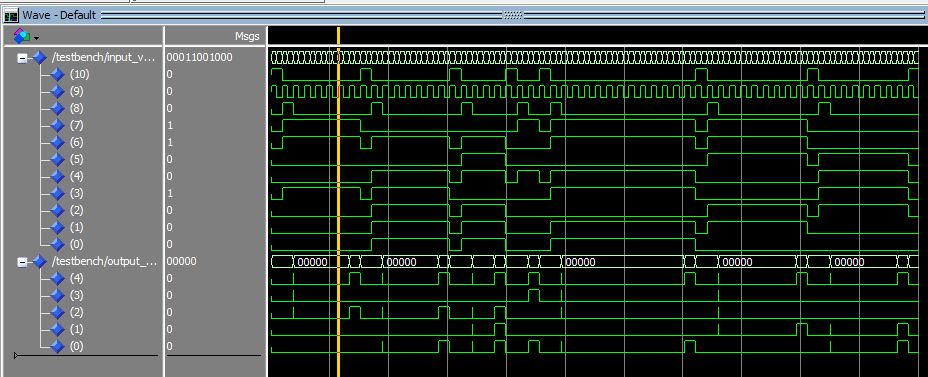
\includegraphics[width=0.9\textwidth]{Screenshot 2026-10-11 173242.png}
  \caption{GCD waveform}
  \label{fig:gcd-waveform}
\end{figure}

\begin{figure}[h]
  \centering
  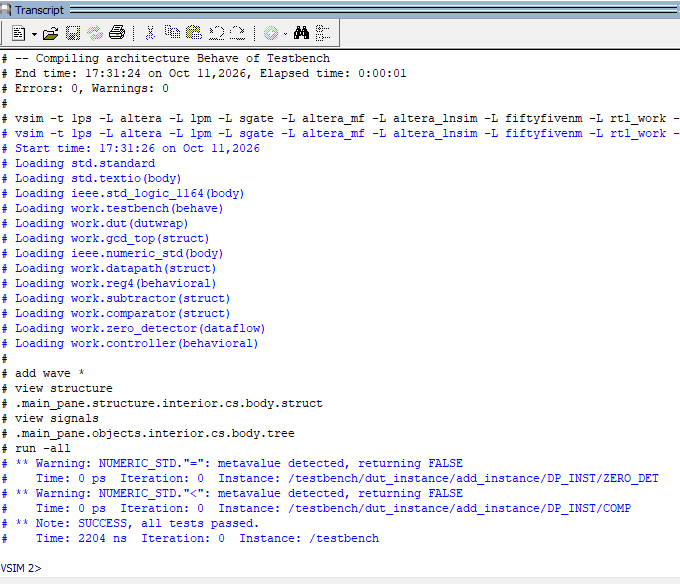
\includegraphics[width=0.9\textwidth]{Screenshot 2026-10-11 173342.png}
  \caption{Transcript}
  \label{fig:transcript}
\end{figure}

\end{document}
